% 第 12 题圆：按固定源 PDF 矢量路径换算（1 pt → 0.03515 cm），取圆心为原点、y 向上。
% 圆心 (594.74,610.27) pt、半径 40.08 pt；直径 AB 水平过圆心；弦 CD 自左上（C 在圆上）经 E（在 AB 上）
% 至右下（D 在圆上，BD=ED）；线段 BD。图中不标圆心、无直角标记、无长度数字。
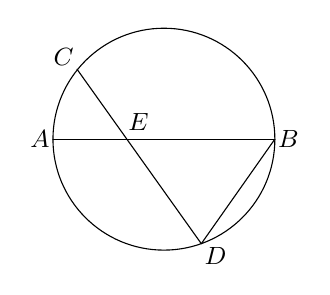
\begin{tikzpicture}[line cap=round,line join=round,font=\small]
\draw (0,0) circle (1.409);
\draw (-1.409,0)--(1.409,0);
\draw (-1.103,0.888)--(0.475,-1.327);
\draw (1.409,0)--(0.475,-1.327);
\node[above left,inner sep=1pt] at (-1.103,0.888) {$C$};
\node[left,inner sep=1pt] at (-1.409,0) {$A$};
\node at (-0.324,0.220) {$E$};
\node[right,inner sep=1pt] at (1.409,0) {$B$};
\node[below right,inner sep=1pt] at (0.475,-1.327) {$D$};
\end{tikzpicture}
